% !TEX encoding = UTF-8
% !TEX TS-program = pdflatex
% !TEX root = tesi.tex
% !TEX spellcheck = it-IT

% PDF/A filecontents
\RequirePackage{filecontents}
\begin{filecontents*}{\jobname.xmpdata}
  \Title{Document’s title}
  \Author{Author’s name}
  \Language{it-IT}
  \Subject{The abstract, or short description.}
  \Keywords{keyword1\sep keyword2\sep keyword3}
\end{filecontents*}

\documentclass[10pt,                    % corpo del font principale
               a4paper,                 % carta A4
               twoside,                 % impagina per fronte-retro
               openright,               % inizio capitoli a destra
               english,                 
               italian,                 
               ]{book}    

%**************************************************************
% Importazione package
%************************************************************** 

\PassOptionsToPackage{dvipsnames}{xcolor} % colori PDF/A

\usepackage{colorprofiles}

\usepackage[a-2b,mathxmp]{pdfx}[2018/12/22]
                                        % configurazione PDF/A
                                        % validare in https://www.pdf-online.com/osa/validate.aspx

%\usepackage{amsmath,amssymb,amsthm}    % matematica

\usepackage[T1]{fontenc}                % codifica dei font:
                                        % NOTA BENE! richiede una distribuzione *completa* di LaTeX
\usepackage{lmodern}

\usepackage[utf8]{inputenc}             % codifica di input; anche [latin1] va bene
                                        % NOTA BENE! va accordata con le preferenze dell'editor

\usepackage[english, italian]{babel}    % per scrivere in italiano e in inglese;
                                        % l'ultima lingua (l'italiano) risulta predefinita

\usepackage{bookmark}                   % segnalibri

\usepackage{caption}                    % didascalie

\usepackage{chngpage,calc}              % centra il frontespizio

\usepackage{csquotes}                   % gestisce automaticamente i caratteri (")

\usepackage{emptypage}                  % pagine vuote senza testatina e piede di pagina

\usepackage{epigraph}			% per epigrafi

\usepackage{eurosym}                    % simbolo dell'euro

%\usepackage{indentfirst}               % rientra il primo paragrafo di ogni sezione

\usepackage{graphicx}                   % immagini

\usepackage{hyperref}                   % collegamenti ipertestuali

\usepackage[binding=5mm]{layaureo}      % margini ottimizzati per l'A4; rilegatura di 5 mm

\usepackage{listings}                   % codici

\usepackage{microtype}                  % microtipografia

\usepackage{mparhack,fixltx2e,relsize}  % finezze tipografiche

\usepackage{nameref}                    % visualizza nome dei riferimenti                                      
\usepackage[font=small]{quoting}        % citazioni

\usepackage{subfig}                     % sottofigure, sottotabelle

\usepackage[italian]{varioref}          % riferimenti completi della pagina

\usepackage{booktabs}                   % tabelle                                       
\usepackage{tabularx}                   % tabelle di larghezza prefissata                                    
\usepackage{longtable}                  % tabelle su più pagine                                        
\usepackage{ltxtable}                   % tabelle su più pagine e adattabili in larghezza

\usepackage[toc, acronym]{glossaries}   % glossario
                                        % per includerlo nel documento bisogna:
                                        % 1. compilare una prima volta tesi.tex;
                                        % 2. eseguire: makeindex -s tesi.ist -t tesi.glg -o tesi.gls tesi.glo
                                        % 3. eseguire: makeindex -s tesi.ist -t tesi.alg -o tesi.acr tesi.acn
                                        % 4. compilare due volte tesi.tex.

\usepackage[backend=biber,style=verbose-ibid,hyperref,backref]{biblatex}
                                        % eccellente pacchetto per la bibliografia; 
                                        % produce uno stile di citazione autore-anno; 
                                        % lo stile "numeric-comp" produce riferimenti numerici
                                        % per includerlo nel documento bisogna:
                                        % 1. compilare una prima volta tesi.tex;
                                        % 2. eseguire: biber tesi
                                        % 3. compilare ancora tesi.tex.

% Autore
\newcommand{\myName}{Mattia Episcopo}
\newcommand{\myTitle}{Sviluppo del frontend di un'applicazione web in React js}

% Tipo di tesi                   
\newcommand{\myDegree}{Tesi di laurea}

% Università             
\newcommand{\myUni}{Università degli Studi di Padova}

% Facoltà       
\newcommand{\myFaculty}{Corso di Laurea in Informatica}

% Dipartimento
\newcommand{\myDepartment}{Dipartimento di Matematica "Tullio Levi-Civita"}

% Titolo del relatore
\newcommand{\profTitle}{Prof.}

% Relatore
\newcommand{\myProf}{Paolo Baldan}

% Luogo
\newcommand{\myLocation}{Padova}

% Anno accademico
\newcommand{\myAA}{2022-2023}

% Data discussione
\newcommand{\myTime}{Febbraio 2023}

%**************************************************************
% Impostazioni di impaginazione
% see: http://wwwcdf.pd.infn.it/AppuntiLinux/a2547.htm
%**************************************************************

\setlength{\parindent}{14pt}   % larghezza rientro della prima riga
\setlength{\parskip}{0pt}   % distanza tra i paragrafi


%**************************************************************
% Impostazioni di biblatex
%**************************************************************
\bibliography{bibliografia} % database di biblatex 

\defbibheading{bibliography} {
  \cleardoublepage
  \phantomsection
  \addcontentsline{toc}{chapter}{\bibname}
  \chapter*{\bibname\markboth{\bibname}{\bibname}}
}

\setlength\bibitemsep{1.5\itemsep} % spazio tra entry

\DeclareBibliographyCategory{opere}
\DeclareBibliographyCategory{web}

\addtocategory{opere}{womak:lean-thinking}
\addtocategory{web}{site:agile-manifesto}

\defbibheading{opere}{\section*{Riferimenti bibliografici}}
\defbibheading{web}{\section*{Siti Web consultati}}


%**************************************************************
% Impostazioni di caption
%**************************************************************
\captionsetup{
  tableposition=top,
  figureposition=bottom,
  font=small,
  format=hang,
  labelfont=bf
}

%**************************************************************
% Impostazioni di glossaries
%**************************************************************
\makeglossaries
% !TEX encoding = UTF-8
% !TEX TS-program = pdflatex
% !TEX root = ../tesi.tex



%**************************************************************
% Acronimi
%**************************************************************
\newacronym[description={\glslink{API}{Application Program Interface}}]
{API}{API}{Application Program Interface}

\newacronym[description={\glslink{uml}{Unified Modeling Language}}]
{uml}{UML}{Unified Modeling Language}

\newacronym[description={\glslink{IDE}{Integrated Development Enviroment}}]
{IDE}{IDE}{Integrated Development Enviroment}

\newacronym[description={\glslink{UI}{User Interface}}]
{UI}{UI}{User Interface}

\newacronym[description={\glslink{MVC}{Model View Controller}}]
{MVC}{MVC}{Model View Controller}

\newacronym[description={\glslink{REST}{REpresentational State Transfer}}]
{REST}{REST}{REpresentational State Transfer}

\newacronym[description={\glslink{JSON}{JavaScript Object Notation}}]
{JSON}{JSON}{JavaScript Object Notation}

\newacronym[description={\glslink{MVVM}{Model-View-ViewModel}}]
{MVVM}{MVVM}{Model-View-ViewModel}

\newacronym[description={\glslink{URL}{Uniform Resource Locator}}]
{URL}{URL}{Uniform Resource Locator}

\newacronym[description={\glslink{HTML}{HyperText Markup Language}}]
{HTML}{HTML}{HyperText Markup Language}

\newacronym[description={\glslink{DOM}{Document Object Model}}]
{DOM}{DOM}{Document Object Model}


%**************************************************************
% Glossario
%**************************************************************
\newglossaryentry{start-up}
{
  name=\glslink{start-up}{start-up},
  text=start-up,
  sort=start-up,
  description={è un'azienda che è nella fase iniziale di avvio delle attività}
}
\newglossaryentry{metadati}
{
  name=\glslink{metadati}{metadati},
  text=metadati,
  sort=metadati,
  description={sono le informazioni che permettono la costruzione dei dati}
}
\newglossaryentry{byte}
{
  name=\glslink{byte}{byte},
  text=byte,
  sort=byte,
  description={è generalmente una sequenza di 8 bit. Con i multipli del byte si identifica l'unità di misura della capacità di memoria}
}
\newglossaryentry{frontend}
{
  name=\glslink{frontend}{frontend},
  text=frontend,
  sort=frontend,
  description={nell'architettura di un applicazione si intende la parte di software visibile all'utente}
}
\newglossaryentry{backend}
{
  name=\glslink{backend}{backend},
  text=backend,
  sort=backend,
  description={nell'architettura di un applicazione si intende la parte di software con la quale l'utente non interagisce direttamente, che generalmente gestisce l'archiviazione dei dati e la  logica di busness}
}
\newglossaryentry{object storage}
{
  name=\glslink{object storage}{object storage},
  text=object storage,
  sort=object storage,
  description={è un architettura per la memorizzazione dei dati, dove questi vengono gestiti come oggetti}
}
\newglossaryentry{libreria}
{
  name=\glslink{libreria}{libreria},
  text=libreria,
  sort=libreria,
  description={è un insieme di funzioni e strutture dati non direttamente eseguibili utilizzati a supporto di un software}
}
\newglossaryentry{form}
{
  name=\glslink{form}{form},
  text=form,
  sort=form,
  description={è la parte di interfaccia utente di un applicazione che consente all'utente l'iserimento di dati}
}
\newglossaryentry{task}
{
  name=\glslink{task}{task},
  text=task,
  sort=task,
  description={in un sistema di organizzazione del lavoro è una specifica attività che fa parte di un progetto}
}
\newglossaryentry{repository}
{
  name=\glslink{repository}{repository},
  text=repository,
  sort=repository,
  description={è un sistema di archiviazione di file e dati utilizzato per gestire il codice di un progetto}
}
\newglossaryentry{workflow}
{
  name=\glslink{workflow}{workflow},
  text=workflow,
  sort=workflow,
  description={nella gestione dei progetti è il flusso di lavoro che un attività deve seguire dalla sua creazione al suo completamento}
}
\newglossaryentry{plugin}
{
  name=\glslink{plugin}{plugin},
  text=plugin,
  sort=plugin,
  description={è un programma a supporto di un altro che ne estende le funzionalità}
}
\newglossaryentry{framework}
{
  name=\glslink{framework}{framework},
  text=framework,
  sort=framework,
  description={è l'architettura logica sulla quale il software viene progettato e realizzato, utilizzato per facilitare lo sviluppo e il mantenimento del codice}
}
\newglossaryentry{jobs}
{
  name=\glslink{jobs}{jobs},
  text=jobs,
  sort=jobs,
  description={nella nostra applicazione con questo termine si intende i procedimenti per i quali è già stato fatto l'upload verso il backend}
}
\newglossaryentry{open-source}
{
  name=\glslink{open-source}{open-source},
  text=open-source,
  sort=open-source,
  description={indica una particolare la licenza di un software, che consente la libera distribuzione la modifica e lo studio}
}
\newglossaryentry{routing}
{
  name=\glslink{routing}{routing},
  text=routing,
  sort=routing,
  description={indica la parte di gestione dell'indirizzamento delle URL e dei percorsi (path) in un applicazione web}
}
\newglossaryentry{endpoint}
{
  name=\glslink{endpoint}{endpoint},
  text=endpoint,
  sort=endpoint,
  description={nella comunicazione frontend-backend tramite API è il punto che il server espone per ricevere richieste ed inviare risposte}
}
\newglossaryentry{sessione}
{
  name=\glslink{sessione}{sessione},
  text=sessione,
  sort=sessione,
  description={nelle applicazioni web, indica l'attività svolta dall'utente da quando si collega all'applicazione tramite browser a quando il collegamento viene chiuso}
}
\newglossaryentry{stato}
{
  name=\glslink{stato}{stato},
  text=stato dell'applicazione,
  sort=stato,
  description={è l'insieme di input di dati e azioni che determinano l'output in un dato momento.}
}
\newglossaryentry{brano}
{
  name=\glslink{brano}{brano},
  text=brano,
  sort=brano,
  description={nelle tracce audio del nostro sistema di registrazione, è la traccia più esterna che può contenere vari sottobrani. Possono essercene più di uno per CD.}
}
\newglossaryentry{sottobrano}
{
  name=\glslink{sottobrano}{sottobrano},
  text=sottobrano,
  sort=sottobrano,
  description={nelle tracce audio del nostro sistema di registrazione, è la traccia più interna che è figlia di un brano. Possono essercene più di una per ogni brano.}
}
\newglossaryentry{canali}
{
  name=\glslink{canali}{canali},
  text=canale audio,
  sort=canale,
  description={nell'aula di tribunale, corrisponde alla registrazione di uno dei microfoni disponibili in aula nei quali uno dei presenti parla. Ad ogni canale audio corrisponde
      una traccia.}
}
\newglossaryentry{traccia mixer}
{
  name=\glslink{traccia mixer}{traccia mixer},
  text=traccia mixer,
  sort=traccia mixer,
  description={nel nostro sistema di registrazione, è la traccia risultato del mixaggio delle tracce corrispondendi ai singoli canali. In particolare ci sono 7 microfoni
      in aula, ognuno viene registrato su una traccia audio, la traccia mixer è quella che registra tutto l'insieme.}
}
\newglossaryentry{parsing}
{
  name=\glslink{parsing}{parsing},
  text=parsing,
  sort=parsing,
  description={significa letteralmente analisi, nel nostro contesto si riferisce all'analisi e all'interpretazione che la libreria creata fa sui metadati che si trovano nel file cronologia}
}
\newglossaryentry{oggetti javascript}
{
  name=\glslink{oggetti javascript}{oggetti javascript},
  text=oggetto javascript,
  sort=oggetto javascript,
  description={sono delle strutture dati che possiamo definire all'interno del nostro codice.}
}
\newglossaryentry{array di oggetti}
{
  name=\glslink{array di oggetti}{array di oggetti},
  text=array di oggetti,
  sort=array di oggetti,
  description={sono delle collezioni non ordinate di oggetti javascript, sulle quali possiamo eseguire operazioni di vario tipo, aggiungere/rimuovere/modificare dati per esempio}
}

%%%%%%%%%%%%%%%%%%%%%%%%%%%%%%%%%%%%%%%%%%%%%%%%%%%%%%%%%
% \newglossaryentry{apig}
% {
%   name=\glslink{api}{API},
%   text=Application Program Interface,
%   sort=api,
%   description={in informatica con il termine \emph{Application Programming Interface API} (ing. interfaccia di programmazione di un'applicazione) si indica ogni insieme di procedure disponibili al programmatore, di solito raggruppate a formare un set di strumenti specifici per l'espletamento di un determinato compito all'interno di un certo programma. La finalità è ottenere un'astrazione, di solito tra l'hardware e il programmatore o tra software a basso e quello ad alto livello semplificando così il lavoro di programmazione}
% }

% \newglossaryentry{umlg}
% {
%   name=\glslink{uml}{UML},
%   text=UML,
%   sort=uml,
%   description={in ingegneria del software \emph{UML, Unified Modeling Language} (ing. linguaggio di modellazione unificato) è un linguaggio di modellazione e specifica basato sul paradigma object-oriented. L'\emph{UML} svolge un'importantissima funzione di ``lingua franca'' nella comunità della progettazione e programmazione a oggetti. Gran parte della letteratura di settore usa tale linguaggio per descrivere soluzioni analitiche e progettuali in modo sintetico e comprensibile a un vasto pubblico}
% }

 % database di termini


%**************************************************************
% Impostazioni di graphicx
%**************************************************************
\graphicspath{{immagini/}} % cartella dove sono riposte le immagini


%**************************************************************
% Impostazioni di hyperref
%**************************************************************
\hypersetup{
  %hyperfootnotes=false,
  %pdfpagelabels,
  %draft,	% = elimina tutti i link (utile per stampe in bianco e nero)
  colorlinks=true,
  linktocpage=true,
  pdfstartpage=1,
  pdfstartview=,
  % decommenta la riga seguente per avere link in nero (per esempio per la stampa in bianco e nero)
  %colorlinks=false, linktocpage=false, pdfborder={0 0 0}, pdfstartpage=1, pdfstartview=FitV,
  breaklinks=true,
  pdfpagemode=UseNone,
  pageanchor=true,
  pdfpagemode=UseOutlines,
  plainpages=false,
  bookmarksnumbered,
  bookmarksopen=true,
  bookmarksopenlevel=1,
  hypertexnames=true,
  pdfhighlight=/O,
  %nesting=true,
  %frenchlinks,
  urlcolor=webbrown,
  linkcolor=RoyalBlue,
  citecolor=webgreen,
  %pagecolor=RoyalBlue,
  %urlcolor=Black, linkcolor=Black, citecolor=Black, %pagecolor=Black,
  pdftitle={\myTitle},
  pdfauthor={\textcopyright\ \myName, \myUni, \myFaculty},
  pdfsubject={},
  pdfkeywords={},
  pdfcreator={pdfLaTeX},
  pdfproducer={LaTeX}
}

%**************************************************************
% Impostazioni di itemize
%**************************************************************
\renewcommand{\labelitemi}{$\ast$}

%\renewcommand{\labelitemi}{$\bullet$}
%\renewcommand{\labelitemii}{$\cdot$}
%\renewcommand{\labelitemiii}{$\diamond$}
%\renewcommand{\labelitemiv}{$\ast$}


%**************************************************************
% Impostazioni di listings
%**************************************************************
\lstset{
  language=[LaTeX]Tex,%C++,
  keywordstyle=\color{RoyalBlue}, %\bfseries,
  basicstyle=\small\ttfamily,
  %identifierstyle=\color{NavyBlue},
  commentstyle=\color{Green}\ttfamily,
  stringstyle=\rmfamily,
  numbers=none, %left,%
  numberstyle=\scriptsize, %\tiny
  stepnumber=5,
  numbersep=8pt,
  showstringspaces=false,
  breaklines=true,
  frameround=ftff,
  frame=single
}


%**************************************************************
% Impostazioni di xcolor
%**************************************************************
\definecolor{webgreen}{rgb}{0,.5,0}
\definecolor{webbrown}{rgb}{.6,0,0}


%**************************************************************
% Altro
%**************************************************************

\newcommand{\omissis}{[\dots\negthinspace]} % produce [...]

% eccezioni all'algoritmo di sillabazione
\hyphenation
{
  ma-cro-istru-zio-ne
  gi-ral-din
}

\newcommand{\sectionname}{sezione}
\addto\captionsitalian{\renewcommand{\figurename}{Figura}
  \renewcommand{\tablename}{Tabella}}

\newcommand{\glsfirstoccur}{\ap{{[g]}}}

\newcommand{\intro}[1]{\emph{\textsf{#1}}}

%**************************************************************
% Environment per ``rischi''
%**************************************************************
\newcounter{riskcounter}                % define a counter
\setcounter{riskcounter}{0}             % set the counter to some initial value

%%%% Parameters
% #1: Title
\newenvironment{risk}[1]{
  \refstepcounter{riskcounter}        % increment counter
  \par \noindent                      % start new paragraph
  \textbf{\arabic{riskcounter}. #1}   % display the title before the 
  % content of the environment is displayed 
}{
  \par\medskip
}

\newcommand{\riskname}{Rischio}

\newcommand{\riskdescription}[1]{\textbf{\\Descrizione:} #1.}

\newcommand{\risksolution}[1]{\textbf{\\Soluzione:} #1.}

%**************************************************************
% Environment per ``use case''
%**************************************************************
\newcounter{usecasecounter}             % define a counter
\setcounter{usecasecounter}{0}          % set the counter to some initial value

%%%% Parameters
% #1: ID
% #2: Nome
\newenvironment{usecase}[2]{
  \renewcommand{\theusecasecounter}{\usecasename #1}  % this is where the display of 
  % the counter is overwritten/modified
  \refstepcounter{usecasecounter}             % increment counter
  \vspace{10pt}
  \par \noindent                              % start new paragraph
  {\large \textbf{\usecasename #1: #2}}       % display the title before the 
  % content of the environment is displayed 
  \medskip
}{
  \medskip
}

\newcommand{\usecasename}{UC}

\newcommand{\usecaseactors}[1]{\textbf{\\Attori Principali:} #1. \vspace{4pt}}
\newcommand{\usecasepre}[1]{\textbf{\\Precondizioni:} #1. \vspace{4pt}}
\newcommand{\usecasedesc}[1]{\textbf{\\Descrizione:} #1. \vspace{4pt}}
\newcommand{\usecasepost}[1]{\textbf{\\Postcondizioni:} #1. \vspace{4pt}}
\newcommand{\usecaseprinc}[1]{\textbf{\\Scenario Principale:} #1. \vspace{4pt}}
\newcommand{\usecasealt}[1]{\textbf{\\Scenario Alternativo:} #1. \vspace{4pt}}

%**************************************************************
% Environment per ``namespace description''
%**************************************************************

\newenvironment{namespacedesc}{
  \vspace{10pt}
  \par \noindent                              % start new paragraph
  \begin{description}
    }{
  \end{description}
  \medskip
}

\newcommand{\classdesc}[2]{\item[\textbf{#1:}] #2}


\begin{document}
\frontmatter
% !TEX encoding = UTF-8
% !TEX TS-program = pdflatex
% !TEX root = ../tesi.tex

%**************************************************************
% Frontespizio 
%**************************************************************
\begin{titlepage}

  \begin{center}

    \begin{LARGE}
      \textbf{\myUni}\\
    \end{LARGE}

    \vspace{10pt}

    \begin{Large}
      \textsc{\myDepartment}\\
    \end{Large}

    \vspace{10pt}

    \begin{large}
      \textsc{\myFaculty}\\
    \end{large}

    \vspace{30pt}
    \begin{figure}[htbp]
      \begin{center}
        
\includegraphics[height=6cm]{logo-unipd}
      \end{center}
    \end{figure}
    \vspace{30pt}

    \begin{LARGE}
      \begin{center}
        \textbf{\myTitle}\\
      \end{center}
    \end{LARGE}

    \vspace{10pt}

    \begin{large}
      \textsl{\myDegree}\\
    \end{large}

    \vspace{40pt}

    \begin{large}
      \begin{flushleft}
        \textit{Relatore}\\
        \vspace{5pt}
        \profTitle \myProf
      \end{flushleft}

      \vspace{0pt}

      \begin{flushright}
        \textit{Laureando}\\
        \vspace{5pt}
        \myName
      \end{flushright}
    \end{large}

    \vspace{40pt}

    \line(1, 0){338} \\
    \begin{normalsize}
      \textsc{Anno Accademico \myAA}
    \end{normalsize}

  \end{center}
\end{titlepage}
% !TEX encoding = UTF-8
% !TEX TS-program = pdflatex
% !TEX root = ../tesi.tex

%**************************************************************
% Colophon
%**************************************************************
\clearpage
\phantomsection
\thispagestyle{empty}

\hfill

\vfill

\noindent\myName: \textit{\myTitle,}
\myDegree,
\textcopyright\ \myTime.
% !TEX encoding = UTF-8
% !TEX TS-program = pdflatex
% !TEX root = ../tesi.tex

%**************************************************************
% Dedica
%**************************************************************
\cleardoublepage
\phantomsection
\thispagestyle{empty}
\pdfbookmark{Dedica}{Dedica}

\vspace*{3cm}

\begin{center}
  Lorem ipsum dolor sit amet, consectetuer adipiscing elit. \\ \medskip
  --- Oscar Wilde
\end{center}

\medskip

\begin{center}
  Dedicato a ...
\end{center}
% !TEX encoding = UTF-8
% !TEX TS-program = pdflatex
% !TEX root = ../tesi.tex

%**************************************************************
% Sommario
%**************************************************************
\cleardoublepage
\phantomsection
\pdfbookmark{Sommario}{Sommario}
\begingroup
\let\clearpage\relax
\let\cleardoublepage\relax
\let\cleardoublepage\relax

\chapter*{Sommario}

Il presente documento descrive l'esperienza di stage del laureando Mattia Episcopo presso l'azienda SAI (Synthema Artificial Inteligence) della durata di circa 300 ore.
L'obiettivo dello stage era la realizzazione del frontend di un'applicazione per la gestione di particolari tracce audio e relativi metadati riguardanti le registrazioni dei
procedimenti delle aule di tribunale. Gli obiettivi dello stage erano diversi ma lo scopo finale era la realizzazione della parte frontend con l'utilizzo del framework javascript React.

\endgroup

\vfill


% !TEX encoding = UTF-8
% !TEX TS-program = pdflatex
% !TEX root = ../tesi.tex

%**************************************************************
% Ringraziamenti
%**************************************************************
\cleardoublepage
\phantomsection
\pdfbookmark{Ringraziamenti}{ringraziamenti}

\begin{flushright}{
    \slshape
    "I'm not crazy, my mother had me tested''} \\
  \medskip
  --- Dott. Sheldon Lee Cooper
\end{flushright}


\bigskip

\begingroup
\let\clearpage\relax
\let\cleardoublepage\relax
\let\cleardoublepage\relax

\chapter*{Ringraziamenti}

\noindent \textit{In primis, ringrazio il prof. Paolo Baldan, relatore della mia tesi, per la disponibilità e l'aiuto fornitomi nella stesura di questo elaborato.}\\

\noindent \textit{Ringrazio l'azienda ospitante, Synthema Artificial Intelligence, e in particolare il tutor interno, Giulio Paci che mi ha guidato in questa esperienza.}\\

\bigskip

\noindent\textit{\myLocation, \myTime}
\hfill \myName

\endgroup

% !TEX encoding = UTF-8
% !TEX TS-program = pdflatex
% !TEX root = ../tesi.tex

%**************************************************************
% Indici
%**************************************************************
\cleardoublepage
\pdfbookmark{\contentsname}{tableofcontents}
\setcounter{tocdepth}{2}
\tableofcontents
%\markboth{\contentsname}{\contentsname} 
\clearpage

\begingroup
\let\clearpage\relax
\let\cleardoublepage\relax
\let\cleardoublepage\relax
%*******************************************************
% Elenco delle figure
%*******************************************************    
\phantomsection
\pdfbookmark{\listfigurename}{lof}
\listoffigures

\vspace*{8ex}

%*******************************************************
% Elenco delle tabelle
%*******************************************************
\phantomsection
\pdfbookmark{\listtablename}{lot}
\listoftables

\vspace*{8ex}
\endgroup

\cleardoublepage


\mainmatter
% !TEX encoding = UTF-8
% !TEX TS-program = pdflatex
% !TEX root = ../tesi.tex


%**************************************************************
\chapter{Introduzione}
\label{cap:introduzione}
%**************************************************************

%Introduzione al contesto applicativo.\\

% \noindent Esempio di utilizzo di un termine nel glossario \\
% \gls{api}. \\

% \noindent Esempio di citazione in linea \\
% \cite{site:agile-manifesto}. \\

% \noindent Esempio di citazione nel pie' di pagina \\
% citazione\footcite{womak:lean-thinking} \\

%**************************************************************%
%**************************************************************%
%**************************************************************%
\section{L'azienda}
\begin{figure}[H]
  \centering
  
\includegraphics[width=2cm]{immagini/logo-SAI.jpg}
  \caption{Loso Syntema Artificial Intelligence}
\end{figure}
Synthema Artificial Intelligence (S.AI) è una start-up innovativa che si occupa di ricerca, progettazione, sviluppo, commercializzazione e manutenzione di
prodotti e servizi innovativi ad alto valore tecnologico, basati sull'Internet of Things, la blockchain e su tecniche di Intelligenza Artificiale
(in particolare reti neurali profonde), per l'analisi integrata e la comprensione di dati multimodali da fonti eterogenee (linguaggio naturale sia scritto che
parlato, audio, immagini, video, dati generati da sensori) e per la gestione dei workflow, sia nel settore pubblico che privato.

%**************************************************************%
%**************************************************************%
%**************************************************************%
\section{Introduzione al progetto}
Il progetto nasce dalla necessità dell'azienda di creare un sistema semi-automatico per la creazione di particolari \emph{\gls{ticketg}}\glsfirstoccur. Il sistema è rivolto ai lavoratori della aule di tribunale,
ovvero i fonici, che si occupano di registrare su dei supporti CD quello che avviene nell'aula di un tribunale. Dopo aver registrato la loro parte di giornata nel tribunale di competenza,
devono inserire tutti i dati relativi ai processi a cui hanno assistito nel sistema di memorizzazione della loro azienda. Le registrazioni audio dei fonici si articolano in una \gls{tracciag} per ogni microfono presente in aula
più una traccia mixer che li riassume tutti. La registrazione di queste tracce audio viene impostata ad inizio giornata, facendo corrispondere ad ogni microfono una traccia, per poi non essere più modificata.
Oltre a questo ogni fonico, con il sistema di registrazione presente in aula, può prendere degli appunti in riferimento a quello che succede, magari per alcuni casi particolari che si possono verificare o per ricordarsi i procedimenti a cui ha assistito.
Tutti questi \gls{metadatig} vengono salvati sottoforma di file di testo, questo file riporta tutto quello che è successo durante la registrazione in ordine cronologico, qual'è il microfono attivo e quinid chi sta parlando, se ci sono appunti particolari e così via.
Il lavoro del fonico si conclude poi con il caricamento di tutte le informazioni raccolte in aula sull'apposito sistema aziendale, con l'obiettivo di tenere traccia di tutti i procedimenti che avvengono nell'aula di tribunale.
Questi dati vengono creati come ticket, ogni ticket si compone di un procedimento, che riporta un proprio codice e deve contenere varie informazioni (chi è o chi sono i giudici, imputati, PM ecc ecc).
Questo processo di creazione e caricamento di ticket al momento è molto laborioso per i fonici che devono sostanzialmente fare tutto a mano, l'obiettivo di questo progetto e del relativo prodotto finale è quello di
automatizzare questo processo, in modo che il fonico solo caricando l'intero CD contenente le tracce audio e il file di testo che le riassume visualizzi i vari ticket dei procedimenti a cui ha assistito. Così facendo il nostro prodotto
garantirebbe una notevole diminuzione del tempo di lavoro, una minor percentuale di errori e lascerebbe all'incaricato solamente l'onere di ricontrollare i dati relativi ai ticket automaticamente creati prima di caricarli sul sistema.

%**************************************************************%
%**************************************************************%
%**************************************************************%
\section{Principali problematiche}
Per questo progetto sorgono diverse problematiche che elenco di seguito:
\begin{itemize}
  \item \textbf{conoscenza dell'argomento}: la conoscenza degli argometi processi, giornata in aula, procedimenti risulta abbastanza vaga allo start del progetto;
  \item \textbf{varietà metadati}: i metadati generati dal sistema, che coinvolgono schema delle tracce e appunti del fonico può generare grandi varietà di casi e sottocasi;
  \item \textbf{grandezza dei dati}: i dati da trattare sono molto grandi, basti pensare che ogni ticket deve comprendere tutte le tracce audio di riferimento e ogni procedimento può durare anche svariate ore;
\end{itemize}

%**************************************************************%
%**************************************************************%
%**************************************************************%
\section{Soluzione scelta}
Il progetto pone vari dubbi nella fase di analisi per scegliere la soluzione migliore, che sia allo stesso tempo veloce nel caricamento dei dati e nella creazione dei ticket ma
che non perda informazioni importanti, visto la sensibilità dei dati trattati. Viene scelto per questo progetto di creare un'applicazione inizialmente web ma con la possibilità
di renderla desktop in futuro. L'applicazione sarà formata da un \gls{backendg} che servirà per tenere traccia delle informazioni che realmente servono per creare un ticket, e un \gls{frontendg}
che servirà principalmente per la composizione delle informazioni da passare al backend.
In questo modo ogni volta che un CD viene caricato non viene interamente mandato al server, ma rimane in gestione al frontend che ne elabora i dati e li gestisce seguendo le preferenze
dell'utente, prima di passare solo i dati necessari al backend. Per la memorizzazione dei file invece la strada pensata in fase di analisi è l'utilizzo di un client (\gls{object-storageg})
esterno dove fare l'upload solo delle tracce audio necessarie. L'oggetto del progetto di stage è proprio la parte di frontend di questo sistema pensato per agevolare il lavoro dei
collaboratori delle aule di tribunale. Riassumendo, le soluzioni scelte a fronte delle principali problematiche riscontrate sono:
\begin{itemize}
  \item \textbf{conoscenza dell'argomento}: abbondante fase di studio iniziale e documentazione sull'argometo;
  \item \textbf{varietà metadati}:
        \begin{itemize}
          \item \textbf{libreria apposita}: creazione di una libreria interna apposita con l'unica funzione di comprendere la maggior parte dei casi dei metadati trovati;
          \item \textbf{editing metadati}: possibilità di editare i metadati dopo che sono stati letti dalla nostra applicazione, per dare la possibilità ai fonici di modificarli in fase di verifica della creazione ticket;
        \end{itemize}
  \item \textbf{grandezza dei dati}:
        \begin{itemize}
          \item \textbf{gestione nel frontend}: gestire i dati nel frontend senza dover spostare tutte le tracce audio sul server prima di capire quali servano realmente alla creazione dei ticket;
          \item \textbf{object storage}: upload delle sole tracce audio che sono necessarie direttamente su un apposito object storage senza dover passarle al backend;
        \end{itemize}
\end{itemize}

%**************************************************************%
%**************************************************************%
%**************************************************************%
\section{Descrizione del prodotto ottenuto}
Il prodotto finale ottenuto si discosta leggermente da quello inizialmente pensato, infatti è stata soltanto abbozzata la costruzione del ticket vero e proprio per motivi legati alle
tempistiche dello stage e per dare la precedenza agli obiettivi obbligatori e desiderabili dello stage stesso.
L'applicazione finale risulta un buon punto di partenza per costruire la restante parte del prodotto. Il prodotto ottenuto ha come inizio l'autenticazione dell'utente con
la maschera di login, in modo che l'accesso a tutte le operazioni sia consentito solo agli utenti autorizzati. L'applicazione nello stato finale presenta le seguenti funzionalità:
\begin{itemize}
  \item \textbf{caricamento dei dati}: l'utente può caricare i dati sull'applicazione scegliendo se caricare interi CD di registrazioni o singoli file, questa seconda funzionalità
        risulta molto utile nel caso l'utente intenda aggiungere singoli file dopo che ha caricato l'intero CD, per gestire manualmente eventuali mancanze.
  \item \textbf{visualizzazione dati}: l'utente ha a disposizione la visualizzazione dei dati caricati in due versioni, in un completo elenco dei file con i relativi metadati associati
        o in un elenco dei procedimenti che il sistema ha rilevato interpretando i metadati.
  \item \textbf{compilazione automatica form}: i \gls{formg} con i codici dei procedimenti risultano automaticamente compilati dopo che la \gls{libreriag} ha interpretato i metadati in fasi di caricamento delle registrazioni.
  \item \textbf{riproduzione audio dei file}: nella pagina di visualizzazione dei file l'utente ha la possibilità di riprodurre ogni traccia audio caricata.
  \item \textbf{visulizzazione metadati del file}: grazie all'interpretazione dei metadati, per ogni file caricato è possibile vedere tutte le informazioni che ha a disposizione,
        nello specifico, l'utente, oltre a trovare tutti i procedimenti rilevati dalla libreria, può visualizzare tutti gli interventi e le annotazioni che sono state rilevate.
  \item \textbf{caricamento procedimenti}: dopo la revisione dei dati caricati, i procedimenti ritenuti validi possono essere facilmente caricati sul Backend, insieme all'upload dei relativi file sull'object storage.
  \item \textbf{riepilogo dati salvati}: l'utente può visulizzare la lista dei procedimenti dei quali è già stato fatto l'upload e andare nel dettaglio del singolo procedimento per visualizzare le informazioni complete.
\end{itemize}


%**************************************************************%
%**************************************************************%
%**************************************************************%
\section{Strumenti utilizzati}
L'azienda usa un'infrastruttura già collaudata della quale fanno parte sistemi di versionamento del codice, strumenti per l'organizzazione del lavoro e per la comunicazione all'interno del gruppo di lavoro.
Di seguito una panoramica dettagliata degli strumenti utilizzati per lavorare nel \gls{team di sviluppatorig} dell'azienda.

%**************************************************************%
\subsection*{Slack}
\begin{figure}[H]
  \centering
  
\includegraphics[width=2cm]{immagini/logo-Slack.jpg}
  \caption{Logo Syntema Artificial Intelligence}
\end{figure}
E lo strumento che viene usato per la collaborazione aziendale, permette di vedere lo stato degli utenti (sviluppatorei dell'azienda
nel nostro caso) se disponibili o assenti al momento. Questa applicazione da la possibilità di comunicare singolarmente con gli altri
partecipanti oppure in piccoli gruppi divisi per progetto. Permette in oltre la condivisione dei file, molto utile nelle
comunicazioni veloci.

%**************************************************************%
\subsection*{Jira}
\begin{figure}[H]
  \centering
  
\includegraphics[width=2cm]{immagini/logo-jira.jpg}
  \caption{Logo jira}
\end{figure}
Jira è lo strumento che l'azienda usa per l'organizzazione del lavoro. Permette di creare vari progetti, e per ogni progetto consente la
creazione dei relativi ticket. In base alla metodologia di lavoro che si sceglie di utilizzare lo strumento permette di adottarla in tutto.
Nel nostro caso la scelta aziendale è il metodo \gls{SCRUM} e questo strumento consente la creazione degli sprint, è fornito di un backlog, ha
una bacheca personalizzata per ogni utente che consente di vedere lo stato di avanzamento dei ticket di interesse. Inoltre consente di creare
report sull'andamento degli sprint oppure su alcuni periodi, cosa molto utile per tracciare la guida nel miglioramento aziendale.

%**************************************************************%
\subsection*{Gitlab}
\begin{figure}[H]
  \centering
  
\includegraphics[width=2cm]{immagini/logo-Gitlab.jpg}
  \caption{Logo Gitlab}
\end{figure}
Sistema di versionamento dei file di codice usato dall'azienda. Questo strumento si basa su git e consente tutte le operazioni di un \gls{repositoryg} git.
I file vengono condivisi tra tutti gli svilupparori grazie a questo strumento, divisi in repository, uno per ogni progetto sul quale l'azienda lavora.
La linea guida aziendale per l'iutilizzo del sistema GitLab si basa sul \gls{workflowg} denominato feature branching, questo sistema di lavoro
prevede di lasciare il ramo principale (solitamente chiamato main) sempre pulito e con una versione funzionante e testata del prodotto, mentre invece
quanto si vuole lavorare su una nuova feature si crea un nuova ramo partendo da quello principale e una volta che questa feature sarà pronta per essere
revisionata e integrata con quella principale si chiederà una \gls{merge requestg} di questo feature branch sul \gls{branchg} principale.
Il mantenimento dei file di codice sul repository si basa sulla regola aziendale 1 modifica - 1 \gls{commitg} - 1 file, ovvero si predilige che ogni branch che lo sviluppatore crea per sviluppare la relativa feature
sia composto da commit che riguardano soltato un file con la relativa modifica.

%**************************************************************%
\subsection*{VS Code}
\begin{figure}[H]
  \centering
  
\includegraphics[width=2cm]{immagini/logo-VSCode.jpg}
  \caption{Logo VS code}
\end{figure}
E l'\gls{IDE} di lavoro utilizzato per sviluppare il locale. Questo strumento è completo di tutto quello che serve per lo sviluppo del prodotto.
Esso infatti consente di sviluppare nei linguaggi che interessano il progetto, aiutando con vari plugin per il riconoscimento del codice,
aiutando così lo sviluppatore a lavorare più velocemente e in modo più intuitivo. Inoltre è competamente integrato con i sistemi di
versionamento, in particolare nel nostro caso con GitLab. Oltre a queste funzionalità consente di utilizzare plugin per la pulizia del
codice, che settati in maniera corretta permettono di rimanere sempre fedeli alle regole aziendali automaticamente ad ogni salvataggio.

%**************************************************************%
\subsection*{Jitsi}
\begin{figure}[H]
  \centering
  
\includegraphics[width=2cm]{immagini/logo-Jitsi.jpg}
  \caption{Logo Jitsi}
\end{figure}
E lo strumento che l'azienda utilizza per le riunioni in \gls{videocallg} settimanali ma anche per quelle individuali che dovessero essere necessarie
in qualsiasi momento.

%**************************************************************%
\subsection*{SCRUM}
\begin{figure}[H]
  \centering
  
\includegraphics[width=2cm]{immagini/logo-SCRUM.jpg}
  \caption{Logo SCRUM}
\end{figure}
\gls{SCRUM} è il \gls{frameworkg} che l'azienda segue per il lavoro in gruppo sui vari progetti. Questo framework molto diffuso per lo sviluppo software in
team si basa su \gls{sprintg} di durata breve che mirano al completamento dei \gls{taskg} assegnati, il ripetersi temporale di questi sprint porta l'avanzamento
del prodotto. Nel nostro caso particolare quella che segue l'azienda è una versione personalizzata di questo framework. Il funzionamento è spiegato di seguito.
\begin{itemize}
  \item Durata degli sprint: normalmente una settimana;
  \item Meeting del lunedì:
        \begin{itemize}
          \item ognuno da una rapida panoramica per tenere tutti aggiornati su quello che ha svolto nella settimana precendente;
          \item si discutono e assegnano i task che si trovavano nel backlog per lo sprint seguente;
          \item rapida retrospettiva per valutazioni critiche dello sprint appena terminato;
        \end{itemize}
  \item Stati dei task da svolgere:
        \begin{itemize}
          \item da completare: nel corrente sprint ma nessuno ci sta ancora lavorando;
          \item in corso: qualcuno sta lavorando a questo task;
          \item pronto per la revisione: il task è stato completato, si attende che l'incaricato revisioni il codice e faccia il merge nel ramo principale;
          \item completato: il task è stato revisionato e integrato nel ramo principale;
          \item bloccato: per qualche ragione il task è bloccato, si scrive il motivo per il quale non può essere proseguito e se è necessario parlarne con qualcuno;
          \item da posticipare: il task deve essere riposto nel backlog e ripianificato per un altro sprint;
        \end{itemize}
\end{itemize}

%**************************************************************%
%**************************************************************%
%**************************************************************%
\section{Organizzazione del testo}

\begin{description}
  \item[{\hyperref[cap:descrizione-stage]{Il secondo capitolo}}] approfondisce la descrizione dello stage come è stato pianificato, quali sono gli oiettivi ed altri dettagli

  \item[{\hyperref[cap:analisi-requisiti]{Il terzo capitolo}}] approfondisce l'analisi dei requisiti in modo tecnico descrive come è stata svolta la fase di analisi

  \item[{\hyperref[cap:progettazione]{Il quarto capitolo}}] approfondisce la progettazione del prodotto descrivendo tecnicamente come è stata pensata l'architettura

  \item[{\hyperref[cap:realizzazione]{Il quinto capitolo}}] approfondisce la realizzazione del prodotto con la descrizione della fase di codifica e di testing

  \item[{\hyperref[cap:conclusioni]{Nel sesto capitolo}}] descrive le conclusioni valutando criticamente l'esperienza di stage e il prodotto ottenuto
\end{description}

Riguardo la stesura del testo, relativamente al documento sono state adottate le seguenti convenzioni tipografiche:
\begin{itemize}
  \item gli acronimi, le abbreviazioni e i termini ambigui o di uso non comune menzionati vengono definiti nel glossario, situato alla fine del presente documento;
  \item per la prima occorrenza dei termini riportati nel glossario viene utilizzata la seguente nomenclatura: \emph{parola}\glsfirstoccur;
  \item i termini in lingua straniera o facenti parti del gergo tecnico sono evidenziati con il carattere \emph{corsivo}.
\end{itemize}

% !TEX encoding = UTF-8
% !TEX TS-program = pdflatex
% !TEX root = ../tesi.tex

%**************************************************************
\chapter{Descrizione dello stage}
\label{cap:descrizione-stage}
%**************************************************************

In questo capitolo viene descritto come si è pianificato e svolto lo stage presso SAI, introducendo il progetto, considerando gli obiettivi e i possibili rischi.

%**************************************************************%
%**************************************************************%
%**************************************************************%
\section{Analisi preventiva dei rischi}
Nella fase di analisi iniziali si sono individuati i principali rischi a cui si poteva andare incontro e si è proceduto a definire le possibili soluzione per farne fronte.

\begin{risk}{Uso di nuove tecnologie}
  \riskdescription{le tecnologie proposte per la gestione e lo sviluppo del progetto erano per lo più nuove o scarsamente conosciute.}
  \risksolution{è stato previsto un periodo iniziale di studio e formazione su queste tecnologie.}
  \label{risk:new-tecnology}
\end{risk}
\begin{risk}{Modalità di lavoro smart working}
  \riskdescription{lo stage è stato fatto completamente da remoto, e poteva portare ad una possibile mancanza di comunicazione e ad un incertezza nelle attività da svolgere.}
  \risksolution{il tutor aziendale si è reso disponibile a vari meeting nelle prime fasi del progetto e nella formazione iniziale, e rimanendo a disposizione per altri meeting  in caso di dubbi sulle attività da svolgere.}
  \label{risk:smart-working}
\end{risk}

\newpage

%**************************************************************%
%**************************************************************%
%**************************************************************%
\section{Requisiti e obiettivi}

Si farà riferimento ai requisiti secondo le seguenti notazioni:
\begin{itemize}
  \item O per i requisiti obbligatori, vincolanti in quanto obiettivo primario richiesto dal committente;
  \item D per i requisiti desiderabili, non vincolanti o strettamente necessari, ma dal riconoscibile valore aggiunto;
  \item F per i requisiti facoltativi, rappresentanti valore aggiunto non strettamente competitivo.
        Le sigle precedentemente indicate saranno seguite da una coppia sequenziale di numeri, identificativo del requisito.
\end{itemize}

\begin{center}
  \renewcommand{\arraystretch}{1.8} %aumento ampiezza righe
  \begin{tabular}{ |l|l| }
    %    \caption{Tabella del tracciamento dei requisti dello stage}
    %    \label{tab:requisiti-stage}
    \hline
    \textbf{Codice} & \textbf{Descrizione}                                                                \\
    \hline
    O01             & autenticazione mediante server remoto                                               \\
    \hline
    O02             & lettura dati da CD                                                                  \\
    \hline
    O03             & precompilazione di form con i dati caricati da CD                                   \\
    \hline
    O04             & editing dei dati del form                                                           \\
    \hline
    D01             & upload dei dati verso i sistemi esterni                                             \\
    \hline
    D02             & test di unità esaustivi                                                             \\
    \hline
    F01             & possibilità di ascoltare le registrazioni                                           \\
    \hline
    F02             & possibilità di modificare i dati mediante interazioni evolute (per es. drag-n-drop) \\
    \hline
    F03             & realizzazione di un'applicazione desktop con Electron                               \\
    \hline
    F04             & compilazione multipiattaforma dell'applicazione desktop                             \\
    \hline
  \end{tabular}
\end{center}

\newpage

%**************************************************************%
%**************************************************************%
%**************************************************************%
\section{Pianificazione}

La pianificazione, in termini di quantità di ore, sarà distribuita in attività di studio e attività implementative.

Lo stage è stato strutturato in due fasi principali, la prima dedicata alle attività di studio e la seconda alle attività implementative. Di seguito vengono elencate le attività pianificate con la relativa quantità di ore stimata per ogni attività.

\begin{itemize}
  \item Studio delle tecnologie (80 ore)
        \begin{itemize}
          \item Setup di un prototipo di applicazione React e del backend (16 ore);
          \item Studio delle librerie necessarie (React, Redux, JWT, OAuth) (64 ore);
        \end{itemize}
  \item Implementazione prototipo (240 ore)
        \begin{itemize}
          \item Realizzazione dell’interfaccia di login (30 ore);
          \item Implementazione lettura e visualizzazione dei dati da CD (70 ore);
          \item Implementazione editing dei dati letti da CD (70 ore);
          \item Implementazione upload dei dati (30 ore);
          \item Testing dei prodotti realizzati (40ore);
        \end{itemize}
\end{itemize}

Per ogni attività riguardante la fase di implementazione del prototipo è stata prevista anche la relativa attività di testing.
Il tutto viene rappresentato dal seguente dal diagramma di Gantt.
\begin{figure}[H]
  \centering
  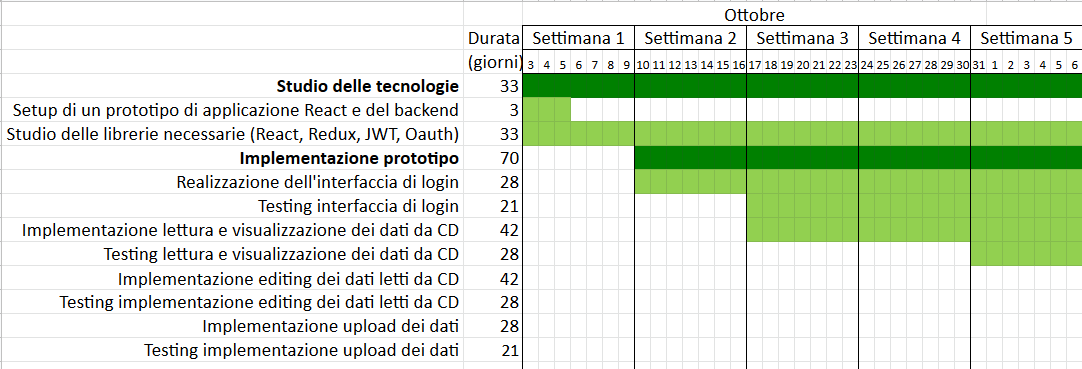
\includegraphics[width=\textwidth]{immagini/gannt1.png}
  \caption{Diagramma di Gantt del piano di lavoro dello stage (parte I)}
\end{figure}
\begin{figure}[H]
  \centering
  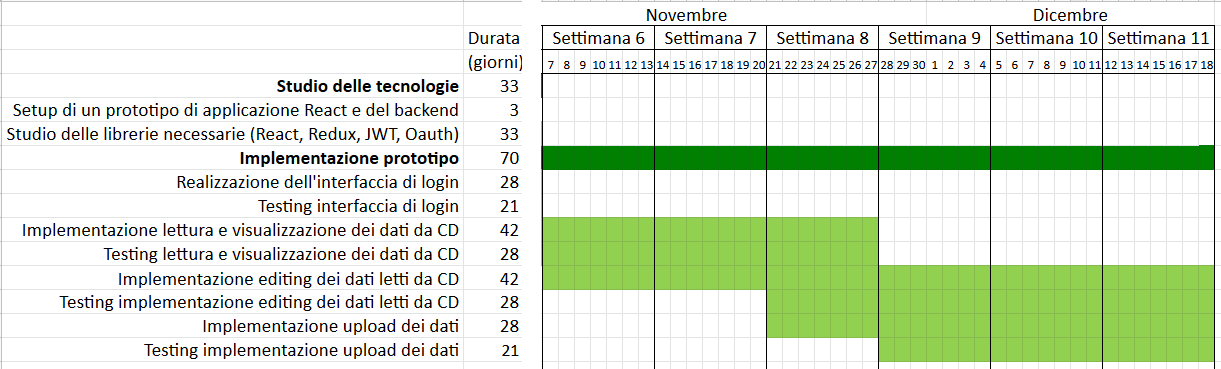
\includegraphics[width=\textwidth]{immagini/gantt2.png}
  \caption{Diagramma di Gantt del piano di lavoro dello stage (parte II)}
\end{figure}

% !TEX encoding = UTF-8
% !TEX TS-program = pdflatex
% !TEX root = ../tesi.tex

%**************************************************************
\chapter{Analisi dei requisiti}
\label{cap:analisi-requisiti}
%**************************************************************

%\intro{Breve introduzione al capitolo}\\

\section{Casi d'uso}

Per lo studio dei casi di utilizzo del prodotto sono stati creati dei diagrammi.
I diagrammi dei casi d'uso (in inglese \emph{Use Case Diagram}) sono diagrammi di tipo \gls{uml} dedicati alla descrizione delle funzioni o servizi offerti da un sistema, così come sono percepiti e utilizzati dagli attori che interagiscono col sistema stesso.
Essendo il progetto finalizzato alla creazione di un tool per l'automazione di un processo, le interazioni da parte dell'utilizzatore devono essere ovviamente ridotte allo stretto necessario. Per questo motivo i diagrammi d'uso risultano semplici e in numero ridotto.
\newpage

% !TEX encoding = UTF-8
% !TEX TS-program = pdflatex
% !TEX root = ../tesi.tex

\subsection{UC1 - Autenticazione}
\begin{itemize}
  \item \textbf{Identificativo}: UC1
  \item \textbf{Nome}: autenticazione
  \item \textbf{Descrizione grafica}:
\end{itemize}

\begin{figure}[H]
  \centering
  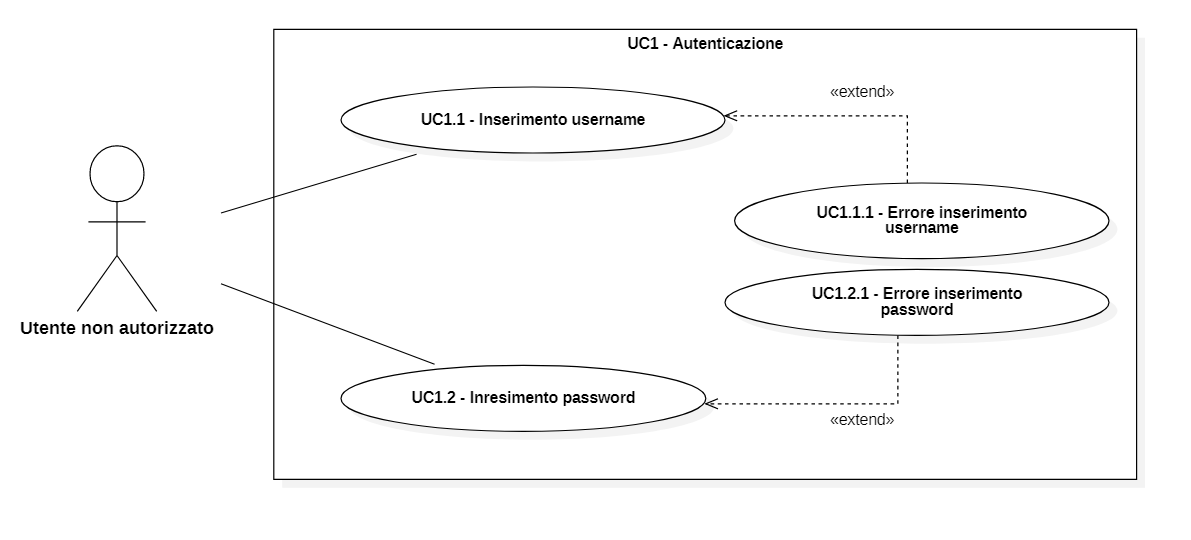
\includegraphics[width=\textwidth]{immagini/usecase/UC1.png}
  \caption{Descrizione grafica caso d'uso UC1}
\end{figure}

\begin{itemize}
  \item \textbf{Attori}
        \begin{itemize}
          \item \textit{Primari}: utente non autorizzato
          \item \textit{Secondari}: Google o Faceebook (???)
        \end{itemize}
  \item \textbf{Precondizione}: l'utente non autenticato si trova sulla pagina di autenticazione.
  \item \textbf{Postcondizione}: l'utente è autenticato.
  \item \textbf{Scenario principale}: l'utente vuole effettuare il login all'applicazione.
  \item \textbf{Scenario secondario}: l'utente non riesce ad autenticarsi a causa di un errore nella procedura. (\textbf{UC1.3})
\end{itemize}

\subsubsection{UC1.1 - Inserimento username}
\begin{itemize}
  \item \textbf{Identificativo}: UC1.1
  \item \textbf{Nome}: inserimento username
  \item \textbf{Descrizione grafica}: (approfondita in UC1)
  \item \textbf{Attori}
        \begin{itemize}
          \item \textit{Primari}: utente non autorizzato
        \end{itemize}
  \item \textbf{Precondizione}: l'utente ha a disposizione una username
  \item \textbf{Postcondizione}: l'utente ha inserito la username.
  \item \textbf{Scenario principale}: l'utente inserisce la username nell'apposito campo di input.
  \item \textbf{Scenario secondario}: l'utente ha inserito una username non corretta che causa un errore. (\textbf{UC1.3})
\end{itemize}

\subsubsection{UC1.1.1 - Errore inserimento username}
\begin{itemize}
  \item \textbf{Identificativo}: UC1.1.1
  \item \textbf{Nome}: errore inserimento username
  \item \textbf{Descrizione grafica}: (approfondita in UC1)
  \item \textbf{Attori}
        \begin{itemize}
          \item \textit{Primari}: utente non autorizzato
        \end{itemize}
  \item \textbf{Precondizione}: la username inserita dall'utente non è correttta.
  \item \textbf{Postcondizione}: l'errore viene mostrato all'utente.
  \item \textbf{Scenario principale}: l'utente inserisce una username non corretta, il sistema segnala l'errore all'utente e mostra nuovamente la maschera di login.
\end{itemize}

\subsubsection{UC1.2 - Inserimento password}
\begin{itemize}
  \item \textbf{Identificativo}: UC1.1
  \item \textbf{Nome}: inserimento password
  \item \textbf{Descrizione grafica}: (approfondita in UC1)
  \item \textbf{Attori}
        \begin{itemize}
          \item \textit{Primari}: utente non autorizzato
        \end{itemize}
  \item \textbf{Precondizione}: l'utente ha a disposizione una password
  \item \textbf{Postcondizione}: l'utente ha inserito la password.
  \item \textbf{Scenario principale}: l'utente inserisce la password nell'apposito campo di input.
  \item \textbf{Scenario secondario}: l'utente ha inserito una password non corretta che causa un errore. (\textbf{UC1.3})
\end{itemize}

\subsubsection{UC1.2.1 - Errore inserimento password}
\begin{itemize}
  \item \textbf{Identificativo}: UC1.2.1
  \item \textbf{Nome}: errore inserimento password
  \item \textbf{Descrizione grafica}: (approfondita in UC1)
  \item \textbf{Attori}
        \begin{itemize}
          \item \textit{Primari}: utente non autorizzato
        \end{itemize}
  \item \textbf{Precondizione}: la password inserita dall'utente non è correttta.
  \item \textbf{Postcondizione}: l'errore viene mostrato all'utente.
  \item \textbf{Scenario principale}: l'utente inserisce una password non corretta, il sistema segnala l'errore all'utente e mostra nuovamente la maschera di login.
\end{itemize}

% \subsubsection{UC1.3 - Errore autenticazione}
% \begin{itemize}
%   \item \textbf{Identificativo}: UC1.3
%   \item \textbf{Nome}: errore autenticazione
%   \item \textbf{Descrizione grafica}: (approfondita in UC1)
%   \item \textbf{Attori}
%         \begin{itemize}
%           \item \textit{Primari}: utente non autorizzato
%         \end{itemize}
%   \item \textbf{Precondizione}: il sitema di autenticazione riceve la richiesta da parte dell'utente.
%   \item \textbf{Postcondizione}: il sistema comunica all'utente l'errore avvenuto, viene riproposta la maschera di login.
%   \item \textbf{Scenario principale}: la richiesta di autenticazione non viene gestita dal sistema che comunica l'errore avvenuto all'utente e mostra nuovamente la maschera di login per un nuovo tentativo.
% \end{itemize}
\newpage
% !TEX encoding = UTF-8
% !TEX TS-program = pdflatex
% !TEX root = ../tesi.tex

\subsection{UC2 - Lettura dati da CD}
\begin{itemize}
  \item \textbf{Identificativo}: UC2
  \item \textbf{Nome}: lettura dati da CD
  \item \textbf{Descrizione grafica}:
\end{itemize}

\begin{figure}[H]
  \centering
  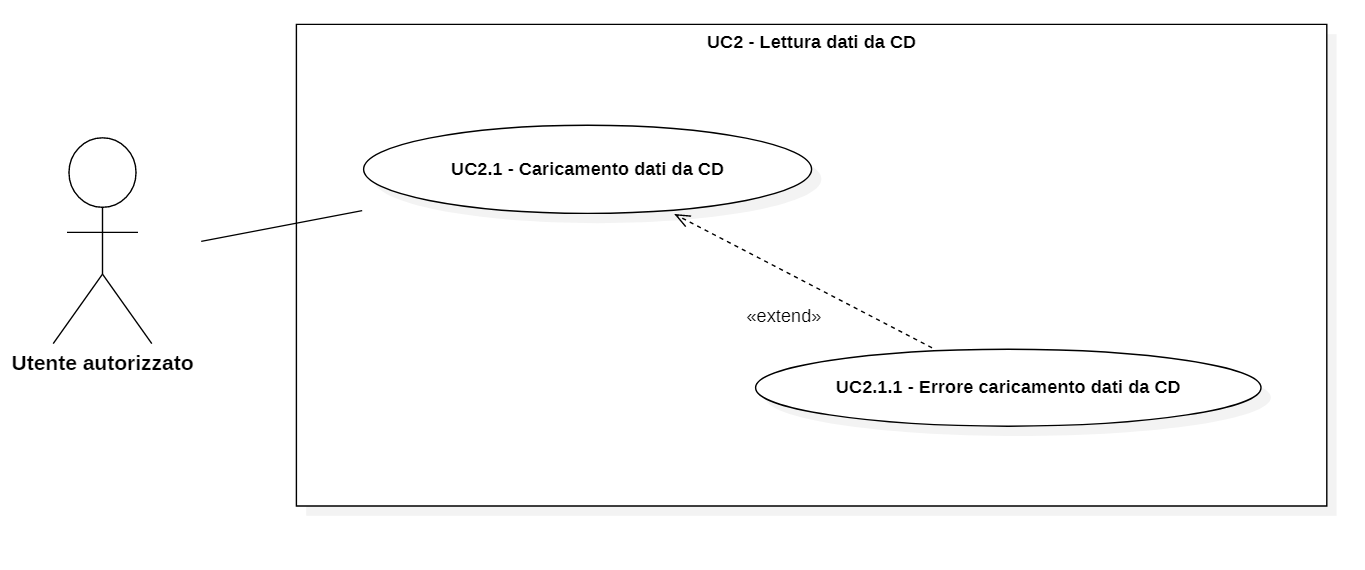
\includegraphics[width=\textwidth]{immagini/usecase/UC2.png}
  \caption{Descrizione grafica caso d'uso UC2}
\end{figure}

\begin{itemize}
  \item \textbf{Attori}
        \begin{itemize}
          \item \textit{Primari}: utente autorizzato
        \end{itemize}
  \item \textbf{Precondizione}: l'utente autorizzato si trova nella pagina per il caricamento dei dati.
  \item \textbf{Postcondizione}: l'utente ha caricato i dati da CD.
  \item \textbf{Scenario principale}: l'utente premendo sull'apposito bottone può caricare i file contenuti nel CD di interesse e li visualizza (\textbf{UC3}).
\end{itemize}

\subsubsection{UC2.1 - Caricamento dati da CD}
\begin{itemize}
  \item \textbf{Identificativo}: UC2.1
  \item \textbf{Nome}: caricamento dati da CD
  \item \textbf{Descrizione grafica}: (approfondita in UC2)
  \item \textbf{Attori}
        \begin{itemize}
          \item \textit{Primari}: utente autorizzato
        \end{itemize}
  \item \textbf{Precondizione}: l'utente ha richiesto il caricamento di una cartella contenente i file del CD.
  \item \textbf{Postcondizione}: i file sono stati caricati nell'applicazione.
  \item \textbf{Scenario principale}: l'utente richiede il caricamento di una cartella contenente i file del CD premendo sull'apposito bottone.
  \item \item \textbf{Scenario secondario}: il sistema riscontra un errore nella procedura di caricamento dei dati. (\textbf{UC2.1})
\end{itemize}

\subsubsection{UC2.1.1 - Errore caricamento dati da CD}
\begin{itemize}
  \item \textbf{Identificativo}: UC2.1
  \item \textbf{Nome}: errore caricamento dati da CD
  \item \textbf{Descrizione grafica}: (approfondita in UC2)
  \item \textbf{Attori}
        \begin{itemize}
          \item \textit{Primari}: utente autorizzato
        \end{itemize}
  \item \textbf{Precondizione}: l'utente ha tentato di caricare i dati.
  \item \textbf{Postcondizione}: l'errore viene mostrato all'utente.
  \item \textbf{Scenario principale}: il sistema non è riuscito a gestire la richiesta di caricamento dei dati da parte dell'utente.
\end{itemize}
\newpage
% !TEX encoding = UTF-8
% !TEX TS-program = pdflatex
% !TEX root = ../tesi.tex

\subsection{UC3 - Visualizzazione file}
\begin{itemize}
  \item \textbf{Identificativo}: UC3
  \item \textbf{Nome}: visualizzazione file
  \item \textbf{Descrizione grafica}:
\end{itemize}

\begin{figure}[h]
  \centering
  %  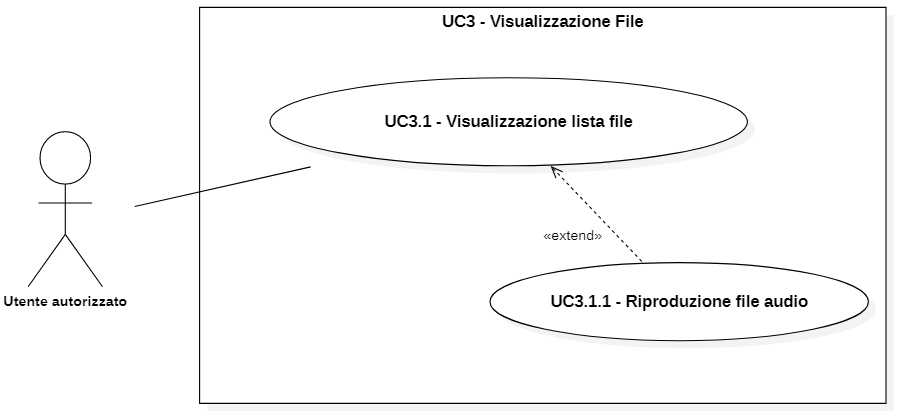
\includegraphics[scale=0.50]{images/UC3.png}
  \caption{Descrizione grafica caso d'uso UC3}
\end{figure}

\begin{itemize}
  \item \textbf{Attori}
        \begin{itemize}
          \item \textit{Primari}: utente autorizzato
        \end{itemize}
  \item \textbf{Precondizione}: l'utente si trova sulla pagina per il caricamento dati, che ha già effettuato correttamente.
  \item \textbf{Postcondizione}: l'utente visualizza i file e i relativi metadati caricati.
  \item \textbf{Scenario principale}: l'utente ha caricato correttamente i dati, questi vengono visualizzati con una lista di file ognuno con i relativi metadati.
  \item \textbf{Scenario secondario}: l'utente può visualizzare ed elaborare i metadati relativi ad ogni file \textbf{UC5}.
\end{itemize}

\subsubsection{UC3.1 - Visualizzazione lista file}
\begin{itemize}
  \item \textbf{Identificativo}: UC3.1
  \item \textbf{Nome}: visualizzazione lista file
  \item \textbf{Descrizione grafica}: (approfondita in UC3)
  \item \textbf{Attori}
        \begin{itemize}
          \item \textit{Primari}: utente autorizzato
        \end{itemize}
  \item \textbf{Precondizione}: l'utente si trova sulla pagina per il caricamento dati, che ha già effettuato correttamente.
  \item \textbf{Postcondizione}: l'utente visualizza la lista dei file ognuno con i relativi metadati.
  \item \textbf{Scenario principale}: l'utente visualizza la lista dei file e può visualizzare la lista dei metadati associati.
  \item \textbf{Scenario secondario}: l'utente può riprodurre i file audio \textbf{UC3.1.1}.
\end{itemize}

\subsubsection{UC3.1.1 - Riproduzione audio file}
\begin{itemize}
  \item \textbf{Identificativo}: UC3.1.1
  \item \textbf{Nome}: riproduzione audio file
  \item \textbf{Descrizione grafica}: (approfondita in UC3)
  \item \textbf{Attori}
        \begin{itemize}
          \item \textit{Primari}: utente autorizzato
        \end{itemize}
  \item \textbf{Precondizione}: l'utente si trova sulla pagina per il caricamento dati, che ha già effettuato correttamente.
  \item \textbf{Postcondizione}: il file audio viene riprodotto.
  \item \textbf{Scenario principale}: l'utente comanda il riproduttore audio con gli appositi comandi play/pause.
\end{itemize}

[Manca visualizzazione/modifica codici procedimenti da capire come gestire questo caso d'uso]
% !TEX encoding = UTF-8
% !TEX TS-program = pdflatex
% !TEX root = ../tesi.tex

\begin{usecase}{4}{Visualizzazione Dati ordinati per Procedimenti}
  \usecaseactors{Utente autorizzato}
  \usecasepre{L'utente si trova all'interno dell'applicazione}
  \usecasedesc{Permette la visualizzazione dei dati caricati da CD}
  \usecasepost{L'utente può visualizzare i dati caricati da CD ordinati per procedimenti}
  \label{uc:visualizzazione-dati-procedimenti}
\end{usecase}


\subsection{UC4 - Visualizzazione dati ordinati per procedimenti}
\begin{itemize}
  \item \textbf{Identificativo}: UC4
  \item \textbf{Nome}: visualizzazione dati ordinati per procedimenti
  \item \textbf{Descrizione grafica}:
\end{itemize}

\begin{figure}[h]
  \centering
  %  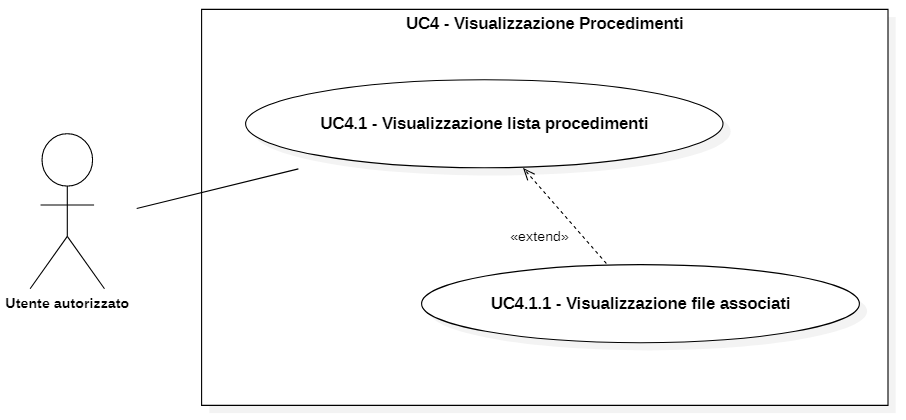
\includegraphics[scale=0.50]{images/UC4.png}
  \caption{Descrizione grafica caso d'uso UC4}
\end{figure}

\begin{itemize}
  \item \textbf{Attori}
        \begin{itemize}
          \item \textit{Primari}: utente autorizzato
        \end{itemize}
  \item \textbf{Precondizione}: l'utente si trova sulla pagina per il caricamento dati, che ha già effettuato correttamente.
  \item \textbf{Postcondizione}: l'utente visualizza i dati caricati sull'applicazione, ordinati per procedimenti.
  \item \textbf{Scenario principale}: l'utente ha caricato correttamente i dati e questi vengono visualizzati ordinati per procedimenti.
\end{itemize}
\newpage
% !TEX encoding = UTF-8
% !TEX TS-program = pdflatex
% !TEX root = ../tesi.tex
\begin{usecase}{5}{Upload Dati}
  \usecaseactors{Utente autorizzato}
  \usecasepre{Lo sviluppatore è entrato nel plug-in di simulazione all'interno dell'IDE}
  \usecasedesc{La finestra di simulazione mette a disposizione i comandi per configurare, registrare o eseguire un test}
  \usecasepost{Il sistema è pronto per permettere una nuova interazione}
  \label{uc:upload-dati}
\end{usecase}

\subsection{UC5 - Upload procedimento}
\begin{itemize}
  \item \textbf{Identificativo}: UC5
  \item \textbf{Nome}: upload procedimento
  \item \textbf{Descrizione grafica}:
\end{itemize}

\begin{figure}[h]
  \centering
  %  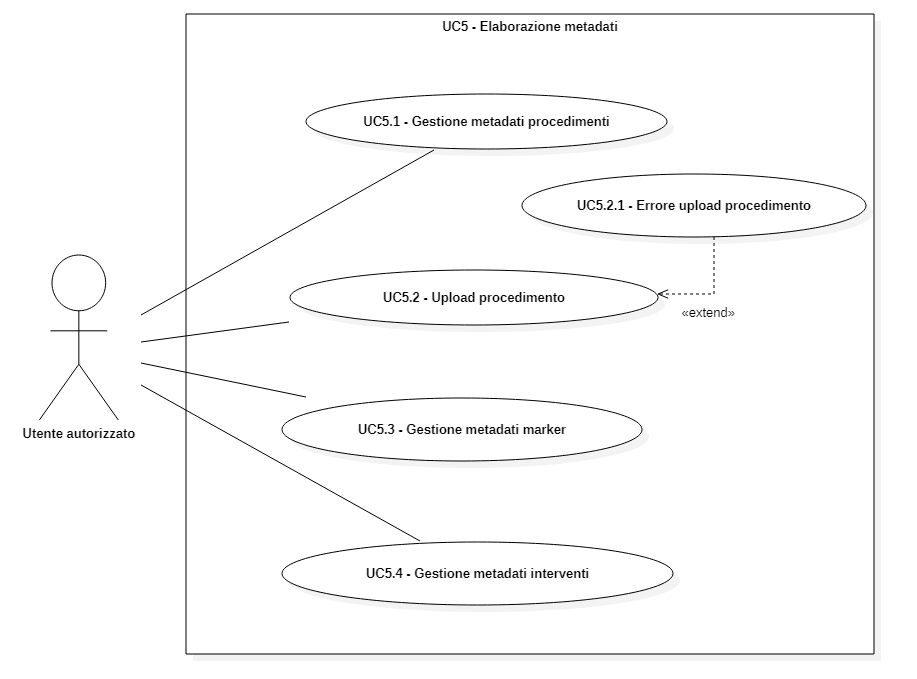
\includegraphics[scale=0.50]{images/UC5.png}
  \caption{Descrizione grafica caso d'uso UC5}
\end{figure}

\begin{itemize}
  \item \textbf{Attori}
        \begin{itemize}
          \item \textit{Primari}: utente autorizzato
        \end{itemize}
  \item \textbf{Precondizione}: l'utente si trova sulla pagina di visualizzazione dei dati.
  \item \textbf{Postcondizione}: l'utente ha caricato il procedimento desiderato e i relativi file.
  \item \textbf{Scenario principale}: l'utente tramite l'apposito bottone per l'upload, carica il procedimento desiderato.
  \item \textbf{Scenario secondario}: la procedura di upload procedimento non va a buon fine e restituisce un errore. (\textbf{UC5.1})
\end{itemize}

\subsubsection{UC5.1 - Errore upload procedimento}
\begin{itemize}
  \item \textbf{Identificativo}: UC5.1
  \item \textbf{Nome}: errore upload procedimento
  \item \textbf{Descrizione grafica}: (approfondita in UC5)
  \item \textbf{Attori}
        \begin{itemize}
          \item \textit{Primari}: utente autorizzato
        \end{itemize}
  \item \textbf{Precondizione}: il sistema non ha gestito correttamente la richiesta di upload procedimento.
  \item \textbf{Postcondizione}: l'errore viene visualizzato sull'applicazione.
  \item \textbf{Scenario principale}: la richiesta di upload procedimento non va a buon fine e l'errore viene mostrato all'utente.
\end{itemize}

% !TEX encoding = UTF-8
% !TEX TS-program = pdflatex
% !TEX root = ../tesi.tex
\begin{usecase}{6}{Visualizzazione Jobs}
  \usecaseactors{Utente autorizzato}
  \usecasepre{L'utente si trova all'interno dell'applicazione}
  \usecasedesc{Permette la visualizzazione dei jobs all'interno dell'applicazione}
  \usecasepost{L'utente può visualizzare i jobs}
  \label{uc:visualizzazione-jobs}
\end{usecase}
\begin{usecase}{7}{Visualizzazione singolo Job}
  \usecaseactors{Utente autorizzato}
  \usecasepre{L'utente si trova sulla pagina di visualizzazione dei jobs}
  \usecasedesc{Permette di visualizzare i dettagli del singolo job}
  \usecasepost{L'utente può visualizzare la pagina del singolo job}
  \label{uc:visualizzazione-job}
\end{usecase}


\subsection{UC6 - Visualizzazione jobs}
\begin{itemize}
  \item \textbf{Identificativo}: UC6
  \item \textbf{Nome}: visualizzazione jobs
  \item \textbf{Descrizione grafica}:
\end{itemize}

\begin{figure}[h]
  \centering
  %  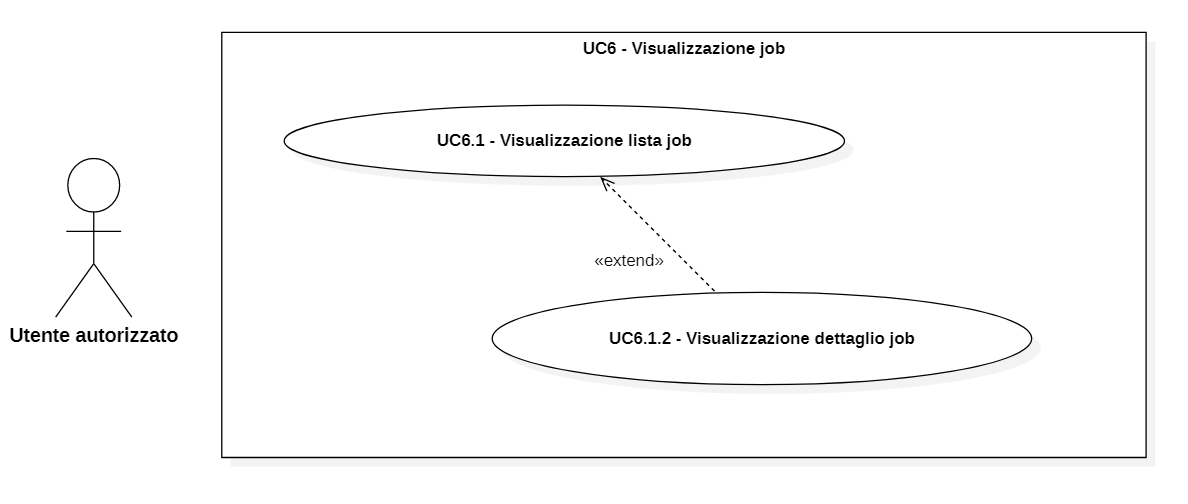
\includegraphics[scale=0.50]{images/UC6.png}
  \caption{Descrizione grafica caso d'uso UC6}
\end{figure}

\begin{itemize}
  \item \textbf{Attori}
        \begin{itemize}
          \item \textit{Primari}: utente autorizzato
        \end{itemize}
  \item \textbf{Precondizione}: l'utente si trova all'interno dell'applicazione e vuole visualizzare la lista dei jobs.
  \item \textbf{Postcondizione}: l'utente visualizza la lista dei jobs.
  \item \textbf{Scenario principale}: l'utente visualizza la lista dei jobs.
  \item \textbf{Scenario secondario}: l'utente può visualizzare il dettaglio di un singolo job premendo sull'apposito link. (\textbf{UC6.1})
\end{itemize}

\subsubsection{UC6.1 - Visualizzazione dettaglio job}
\begin{itemize}
  \item \textbf{Identificativo}: UC6.1
  \item \textbf{Nome}: visualizzazione dettaglio job
  \item \textbf{Descrizione grafica}: (approfondita in UC6)
  \item \textbf{Attori}
        \begin{itemize}
          \item \textit{Primari}: utente autorizzato
        \end{itemize}
  \item \textbf{Precondizione}: l'utente ha premuto sull'apposito link.
  \item \textbf{Postcondizione}: il dettaglio del job viene visualizzato.
  \item \textbf{Scenario principale}: l'utente visualizza tutti i dettagli del singolo job.
\end{itemize}


\section{Tracciamento dei requisiti}

Da un'attenta analisi dei requisiti e degli use case effettuata sul progetto è stata stilata la tabella che traccia i requisiti in rapporto agli use case.\\
Sono stati individuati diversi tipi di requisiti e si è quindi fatto utilizzo di un codice identificativo per distinguerli.\\
Il codice dei requisiti è così strutturato R(F/Q/V)(N/D/O) dove:
\begin{enumerate}
  \item[R =] requisito
  \item[F =] funzionale
  \item[Q =] qualitativo
  \item[V =] di vincolo
  \item[N =] obbligatorio (necessario)
  \item[D =] desiderabile
  \item[F =] facoltativo
\end{enumerate}
Nelle tabelle \ref{tab:requisiti-funzionali} e \ref{tab:requisiti-qualitativi} sono riassunti i requisiti e il loro tracciamento con gli use case delineati in fase di analisi.

\newpage
\renewcommand{\arraystretch}{1.8} %aumento ampiezza righe
\begin{table}%
  \caption{Tabella del tracciamento dei requisti funzionali}
  \label{tab:requisiti-funzionali}
  \begin{tabularx}{\textwidth}{lXl}
    \hline
    \textbf{Requisito} & \textbf{Descrizione}                           & \textbf{Use Case} \\
    \hline
    RFO-1              & autenticazione                                 & UC1               \\
    \hline
    RFO-2              & lettura dati da CD                             & UC2               \\
    \hline
    RFO-3              & visualizzazione dati ordinati per file         & UC3               \\
    \hline
    RFO-4              & visualizzazione dati ordinati per procedimenti & UC4               \\
    \hline
    RFO-5              & gestione dei Marker relativi al file           & UC3               \\
    \hline
    RFO-6              & gestione degli Interventi relativi al file     & UC3               \\
    \hline
    RFD-1              & upload procedimento                            & UC5               \\
    \hline
    RFF-2              & visualizzazione jobs                           & UC6               \\
    \hline
    RFF-1              & riproduzione audio file                        & UC3.1             \\
    \hline
  \end{tabularx}
\end{table}%
\renewcommand{\arraystretch}{1.8} %aumento ampiezza righe
\begin{table}%
  \caption{Tabella del tracciamento dei requisiti qualitativi}
  \label{tab:requisiti-qualitativi}
  \begin{tabularx}{\textwidth}{lXl}
    \hline
    \textbf{Requisito} & \textbf{Descrizione}    & \textbf{Use Case} \\
    \hline
    RQD-1              & test di unità esaustivi & -                 \\
    \hline
  \end{tabularx}
\end{table}%
% !TEX encoding = UTF-8
% !TEX TS-program = pdflatex
% !TEX root = ../tesi.tex

%**************************************************************
\chapter{Progettazione}
\label{cap:progettazione-codifica}
%**************************************************************

\intro{Breve introduzione al capitolo}\\

%**************************************************************
\section{Tecnologie}
\label{sec:tecnologie-strumenti}

Di seguito viene data una panoramica delle tecnologie utilizzate.

\subsection*{Javascript}
JavaScript è un linguaggio di programmazione orientato agli oggetti e agli eventi, comunemente utilizzato nella programmazione Web lato client per la creazione applicazioni web. L'intera applicazione è stata scritta con questo linguaggio.

\subsection*{React}
React è una libreria Javascript utilizzata per implementare interfacce utente (UI) lato frontend. React si basa sul concetto di component, idealmente è una libreria che permette di costruire i propri component come fossere degli elementi HTML del DOM per poi poterli riusare nell'intera applicazione.

\subsection*{Redux \& Redux RTK}
Redux è un contenitore dello stato per le applicazione Javascript. Viene usato per la gestione centralizzata dello stato delle applicazioni sviluppate in React Javascript. In particolare con la sua libreria Redux-Toolkit, permette una gestione dello stato semplice ed efficente.

\subsection*{API rest}
Descrizione Tecnologia 2

\subsection*{JSON}
Markup usato per la pubblicazione dei dati dell’API.

\subsection*{MUI}
Material UI è una libreria React open-source che permette di implementare i Google's Material Design. Essa comprende una collezione di componenti React precostruiti che possono essere facilmente adattati e messi in uso nella UI dell'applicazione.

\subsection*{React Router}
React Router è la libreria standard per il routing in React. Questa libreria permette la navigazione tra le varie viste dell'applicazione , permette di gestire le URL, e mantenere la sincronizzazione tra URL e viste.

\subsection*{Docker}
Docker è un sistema che permette di facilitare il deployment delle applicazioni.

\subsection*{airbnb js guidelines} (???)
Descrizione Tecnologia 2

\subsection*{eslint} (???)

%**************************************************************
\subsection{Architettura dell'applicazione}
L'architettura dell'applicazione era già stata progettata prima dello stage e in piccola parte già esistente.
L'intero sistema si basa sull'interazione tra backend e frontend mediante API rest, con l'auito del gestore di file minIO utilizzato
per la memorizzazione dei file che vengono caricati dell'utente. Il sistema presenta quindi la formazione client-server dove nel server
risiede la parte backend dell'applicativo mentre invece i vari client rappresentano il frontend dell'applicativo.
[disegno generale di front end back end api minio ecc ecc]
\subsubsection*{Backend}
Il backend è un applicazione a se stante scritta interamente in python, con architettura MVC (Model-View-Controller). Questa applicazione
espone delle URL come endpoint per le chiamate REST del client frontend.
\subsubsection*{Frontend}
Il frontend dell'applicazione è la parte che è stata interamente implementata in oggetto allo stage, è l'interfaccia grafica
presentata all'utente.
\subsubsection*{APIrest}
Le API rest sono il tramite tra le due applicazioni, vengono gestite nella parte di frontend con redux-tolkit, e interrogano
il backend sugli appositi endpoint, per poi lasciare al frontend l'interpretazione del risultato. Sono state utilizzate chiamate di
tipo GET e POST. Inoltre una particolare chiamata di tipo PUT viene effettuata dal frontend per l'upload dei file su minIO.
\subsubsection*{MinIO}
%**************************************************************
\subsection{Architettura frontend}
disegno del frontend redux react come lavorano
Il frontend dell'applicazione è stato progettato come una single page application, che mantiene seprarazione tra lo stato e la
user interface.
\subsubsection*{React}
\subsubsection*{Redux}
\subsubsection*{React router}
\subsubsection*{Mui}
%**************************************************************
\section{Progettazione}
\label{sec:progettazione}
viste implementate (jobs, proceeding view, file view), caricamento dati, upload dei dati, un po di come sono state pensate

In sede di progettazione del frontend si è deciso di realizzarlo in javascript, e in particolare usando la libreria react, sfruttando a pieno il riutilizzo del codice che questa libreria permette agevolmente costruendo componenti.
Lo stato del frontend è stato gestito in modo indipendente utilizzando redux, e redux toolkit per sfruttare le API quando è necessario comunicare con il backend.
Per il routing è stata utilizzata la libreria apposita react-router che permette con semplicità di gestire le url e i link all'interno dell'applicazione senza dover usare strumenti esterni al linguaggio.
Graficamente invece, si è scelto di usare MUI per mantenere un interfaccia molto intuitiva, semplice da usare, responsive e con tanti elemente già pronti per essere integrati con React.

Redux permette di creare uno store, dove persistono tutti i dati che vogliamo gestire lato frontend, questo permette di non dover salvare i dati sul server e fare inutili e pesanti chimate ogni volta che si necessita di rappresentare questi dati.
Lo store nel nostro caso particolare è stato usato per memorizzare lato frontend i "dati caricati dall'utente nella fase di caricamento dati da CD".

1) store
2) componenti
3) integrazione componenti
5) routing
4) viste principali

%**************************************************************
\section{Design Pattern utilizzati}
 (??????) tipo observer template se react lo usa... c'è una forma di MVVM in react+redux... posso citare MVC del back end o non frega niente a nessuno?


% !TEX encoding = UTF-8
% !TEX TS-program = pdflatex
% !TEX root = ../tesi.tex

%**************************************************************
\chapter{Realizzazione e testing}
\label{cap:progettazione-codifica}
%**************************************************************

\intro{Breve introduzione al capitolo}\\

%**************************************************************

\section{Codifica}
Come ho agito in fase di codifica, cioè creazione dello store redux, creazione dell'api rtk, creazione dei vari componenti in react, integrazione dei componenti react, interazione tra componenti e stato/store test???
eslint-airbnb style guide utilizzate come standard aziendale
versionamento in gitlab regola aziendale 1 modifica 1 file 1 commit (nella situazione ideale), new file and delete file tutti sullo stesso commit purchè tutti dello stesso tipo
big commit iniziali o di modifiche più sostanziose 1 file 1 commit

Generalmente il flusso della codifica viene gestito in base allo sprint scrum, quindi lunedì retrospettiva su attività fatte, selezione delle attività da fare per lo scritp settimanale e si parte.
il ticket passa dallo stato "da completare" allo stato "in corso"
parlando di react che induce all'uso di componenti riutilizzabili, si è cercato di sfruttare il più possibile questo principio.
creazione di un nuovo componente
integrazione del componente nella vista / nelle viste
creazione dello store redux
creazione delle api redux-toolkit

flusso di lavoro in gitlab, con branch flow.. merge requeste per quando si deve approvare qualche modifica, ticket che passa in stato "da verificare"
se necessita di altre modifiche torna "in corso" altrimenti va in "completato"

parallelismo tra flow di git usato e ticketing jira con metodo scrum
documentazione nei ticket e nelle merge request di tutto quello che è stato fatto
% !TEX encoding = UTF-8
% !TEX TS-program = pdflatex
% !TEX root = ../tesi.tex

%**************************************************************
\chapter{Conclusioni}
\label{cap:conclusioni}
%**************************************************************
\section{Consuntiovo finale}
\label{sec:consuntivo-finale}

\begin{center}
  \renewcommand{\arraystretch}{1.8} %aumento ampiezza righe
  \begin{tabular}{ |p{1cm}|p{2,5cm}|p{8,5cm}| }
    %    \caption{Tabella del tracciamento dei requisti dello stage}
    %    \label{tab:requisiti-stage}
    \hline
    \multicolumn{2}{|c|}{\textbf{Settimana}} & \textbf{Attività}                                                                                                  \\
    \hline
    1                                        & dal 17/10/2022 al 25/10/2022 & autenticazione mediante server remoto                                               \\
    \hline
    2                                        & dal 17/10/2022 al 25/10/2022 & lettura dati da CD                                                                  \\
    \hline
    3                                        & dal 17/10/2022 al 25/10/2022 & precompilazione di form con i dati caricati da CD                                   \\
    \hline
    4                                        & dal 17/10/2022 al 25/10/2022 & editing dei dati del form                                                           \\
    \hline
    5                                        & dal 17/10/2022 al 25/10/2022 & upload dei dati verso i sistemi esterni                                             \\
    \hline
    6                                        & dal 17/10/2022 al 25/10/2022 & test di unità esaustivi                                                             \\
    \hline
    7                                        & dal 17/10/2022 al 25/10/2022 & possibilità di ascoltare le registrazioni                                           \\
    \hline
    8                                        & dal 17/10/2022 al 25/10/2022 & possibilità di modificare i dati mediante interazioni evolute (per es. drag-n-drop) \\
    \hline
    9                                        & dal 17/10/2022 al 25/10/2022 & realizzazione di un'applicazione desktop con Electron                               \\
    \hline
    10                                       & dal 17/10/2022 al 25/10/2022 & compilazione multipiattaforma dell'applicazione desktop                             \\
    \hline
  \end{tabular}
\end{center}

% \subsection*{Orario}

% \subsection*{Sviluppo}

\section{Raggiungimento degli obiettivi}
\label{sec:raggiungimento-obiettivi}
\begin{center}
  \renewcommand{\arraystretch}{1.8} %aumento ampiezza righe
  \begin{tabular}{ |p{1cm}|p{9cm}|p{2cm}| }
    %    \caption{Tabella del tracciamento dei requisti dello stage}
    %    \label{tab:requisiti-stage}
    \hline
    \textbf{Codice} & \textbf{Descrizione}                                                                & \textbf{Stato}          \\
    \hline
    O01             & autenticazione mediante server remoto                                               & soddisfatto             \\
    \hline
    O02             & lettura dati da CD                                                                  & soddisfatto             \\
    \hline
    O03             & precompilazione di form con i dati caricati da CD                                   & soddisfatto             \\
    \hline
    O04             & editing dei dati del form                                                           & soddisfatto             \\
    \hline
    D01             & upload dei dati verso i sistemi esterni                                             & soddisfatto             \\
    \hline
    D02             & test di unità esaustivi                                                             & soddisfatto             \\
    \hline
    F01             & possibilità di ascoltare le registrazioni                                           & soddisfatto             \\
    \hline
    F02             & possibilità di modificare i dati mediante interazioni evolute (per es. drag-n-drop) & non\newline soddisfatto \\
    \hline
    F03             & realizzazione di un'applicazione desktop con Electron                               & non\newline soddisfatto \\
    \hline
    F04             & compilazione multipiattaforma dell'applicazione desktop                             & non\newline soddisfatto \\
    \hline
  \end{tabular}
\end{center}

\section{Prodotto ottenuto}
\label{sec:prodotto-ottenuto}
Alla fine dell'esperienza di stage il prodotto, come già accennato nella parte introduttiva della relazione, si discosta leggermente dal quello che sarà il prodotto finale da
mettere in produzione. Si è deciso per motivi di tempo e di comprensione dell'argomento di realizzare le funzionalità che erano oggetto dello stage in prima battuta e svolgere in seconda
fase tutto quello che riguarda l'integrazione tra le varie parti del frontend, in particolare la creazione del ticket che alla fine dell'esperienza risulta non ancora completata.
Il prodotto non è ancora in produzione, ma è in un buono stato di avanzamento, a giudizio dell'azienda ospitante lo stage, e guardando al futuro si prevede che con qualche altro mese di
lavoro, potrà passare alla fase di collaudo.

\section{Conoscenze acquisite}
\label{sec:conoscenze-acquisite}
Questa esperienza di stage ha avuto grande valore per quanto riguarda l'acquisizione delle conoscenze tecniche e tecnologiche, infatti grazie all'aiuto in partocolare del tutor ma anche
di altri sviluppatore del team dell'azienda ospitante lo stage, posso dire di aver raggiunto una buona conoscenza degli strumenti utilizzati ma anche a lato pratico delle tecnologie
impiegate per lo sviluppo e i test. Guardando nel particolare, per qunato riguarda l'organizzazione aziendale e la gestione del progetto, ho acquisito una conoscenza approfondita nell'
utilizzo del framework SCRUM. Inoltre sempre per quanto riguarda la gestione del codice, un altro personale grande passo in avanti è stato fatto nella comprensione approfondita
di git della maggioranza delle sue funzionalità, in modo specifico per quanto riguarda il workflow utilizzato dall'azienda, il feature branch. A lato sviluppo e testing ovviamente l'apprendimento
è risultato più difficile perchè le tecnologie utilizzate erano completamente nuove in particolare Redux ma anche React, solo per citare le principali, ma in una valutazione retrospettiva
posso dire che il migliramento, nella comprensione dei paradigmi di sviluppo, e delle buone norme di codifica per le tecnologie utilizzate, è stato molto soddisfacente.

\section{Valutazione finale prodotto}
\label{sec:valutazione-finale-prodotto}
Il prodotto finale come detto in precedenza non risulta ancora utilizzato, ma essendo un progetto reale che l'azienda porterà avanti per mettere in seguito in produzione, continuerà ad
essere sviluppato per raggiungere quelli che sono gli obiettivi che l'azienda ha posto nell'analisi iniziale. Alla fine dell'esperienza di stage da parte mia sicuramente resta una piccola parte
di insoddisfazione per non aver raggiunto anche gli obiettivi posti come facoltativi che l'azineda porterà a termine nel prossimo futuro. La principale problematica riscontrata alla fine
dell'esperienza penso di poter dire che è la non conoscenza delle tecnologie utilizzate per lo sviluppo, nonostante un iniziale periodo di studio e prova, prima di iniziare a sviluppare
il prodotto vero e proprio, quando sono arrivato alla fine dello stage la mia conoscenza teorica e pratica è molto migliorata e questo mi fa guardare alla prime fasi di codifica con
insoddisfazione perchè con le conoscenze ora acquisite sicuramente queste parti si potevano svolgere in modo migliore, ecco perchè prima di ultimare lo stage parlando con il tutor ho
proposto varie soluzioni per migliorare la codifica del prodotto, per renderlo più solido, consistente, efficiente, efficace e manutenibile. Tutto questo costerà tempo all'azienda ma
probabilmente sarà del tempo che in futuro verrà risparmiato per eventuali future o manutenzioni da fare. Un altro punto su cui si è discusso con il referente aziendale è quello delle
funzionalità del prodotto, perchè come è normale che sia, in corso di sviluppo le funzinalità inizialmente previste vengono riviste e rivalutate. Per il nostro prodotto tutto quello
che era stato pensato in fase di analisi è stato tenuto come funzionalità da preservare anche per il futuro del prodotto, ma qualche aggiunta è stata pensata per renderlo più veloce e
pratico da utilizzare per i fonici, visto che l'obittivo del prodotto è proprio quello di facilitare il loro lavoro.

\section{Valutazione finale stage}
\label{sec:valutazione-finale-stage}
L'eperienza di stage è stata assolutamente positiva, mi ha dato modo di vedere a lato pratico molte delle cose che avevo visto in modo teorico nel corso degli studi. Ho effettuato lo
stage completamente da remoto, in modalità smart-working, e anche da questo punto di vista sono rimasto molto soddisfatto perchè ho potuto apprezzare il potenziale di questa modalità di
lavoro e secondo la mia opinione spinge maggiormente lo studente in stage a rendersi autonomo dal punto di vista lavorativo, ne migliora le capacità organizzative e consente la flessibilità
rispetto agli orari. In un modo di lavoro dove si guarda più agli obiettivi da raggiungere che al tempo effettivo di lavoro si incorre nel rischio di stimare male le tempistiche per le
attività da svolgere ma allo stesso tempo si rende maggiormente responsabile il lavoratore, e nel lungo periodo si valutano in modo più oggettivo le competenze e le capacità, è una
scelta che continuerei a fare anche nel mio futuro lavorativo. Un grande aiuto l'ho ricevuto dal mio tutor e da altri sviluppatori che con grande pazienza e conoscenze degli
argomenti molto approfondite mi hanno guidato in questo stage, senza mai lasciarmi ad affrontare i problemi del progetto da solo ma rimanendo sempre a disposizione per qualsiasi mio dubbio,
e mi ritengo molto soddisfatto anche per questo dell'azienda scelta per questa esperienza. L'unica vera difficoltà che ho incontrato in questo stage è la poca conoscenza iniziale delle
tecnologie, in particolare di React e ma in parte anche di git, che mi hanno costretto ad un inizio un po lento fatto più che altro di studio e approfondimento delle conoscenze, questo ha
comportato un rallentamento di tutte le attività del progetto, andando un po ad influire sulle tempistiche e il prodotto finale.

\backmatter
\printglossary[type=\acronymtype, title=Acronimi e abbreviazioni, toctitle=Acronimi e abbreviazioni]
\printglossary[type=main, title=Glossario, toctitle=Glossario]
% !TEX encoding = UTF-8
% !TEX TS-program = pdflatex
% !TEX root = ../tesi.tex

%**************************************************************
% Bibliografia
%**************************************************************

\cleardoublepage
\chapter{Bibliografia}

\nocite{*}
% Stampa i riferimenti bibliografici
\printbibliography[heading=subbibliography,title={Riferimenti bibliografici},type=book]

% Stampa i siti web consultati
\printbibliography[heading=subbibliography,title={Siti web consultati},type=online]


\end{document}